\chapter{Mathematical Toolkit}
\label{app:math}

This appendix collects the mathematical habits the book uses: not statistics, but the handful of ideas from calculus, sets and probability that the proofs lean on.
Each entry says what the idea is in plain words, draws it, and names the first place in the book that needs it.
When a chapter marks a step with `(toolkit \ref{sec:math-mvt})', this is where to come.
Nothing here is needed to state a result; everything here is needed to follow a proof.
Later chapters will add entries of their own (vectors and matrices for regression, the chi-squared family for tests) at the end.

\section{Limits of sequences of numbers}
\label{sec:math-limits}

A sequence of numbers $x_1, x_2, x_3, \ldots$ \textbf{converges} to $x$ if the terms eventually stay as close to $x$ as you like.
The definition makes `as close as you like' and `eventually' precise:
\[
\text{for every } \epsilon > 0 \text{ there is an index } N \text{ such that } \abs{x_n - x} < \epsilon \text{ for all } n \geq N.
\]
Read it as a game with an opponent.
The opponent names a tolerance $\epsilon$, any positive number, however small.
You must answer with an index $N$ past which every term of the sequence is within $\epsilon$ of $x$.
If you can always answer, the sequence converges.
The order of the two moves is the whole content: $\epsilon$ is chosen first and $N$ is allowed to depend on it, which is why a smaller $\epsilon$ is usually met with a larger $N$ (\cref{fig:tk-epsilon}).
Writing the moves in the other order (`there is an $N$ that works for every $\epsilon$') would say the sequence is eventually \textit{equal} to $x$, a much stronger and usually false statement.
The left of \cref{fig:tk-epsilon} plays the game for $x_n = 2 + (-1)^n/\sqrt{n}$ with two tolerances: for $\epsilon = 0.3$ every term past $N = 12$ is inside the band, and for $\epsilon = 0.1$ you need $N = 101$ (at $n = 100$ the term sits exactly on the band's edge, and the definition asks for strictly inside).
The right draws the index that works as a function of the tolerance; it climbs as $\epsilon$ shrinks, and convergence means the staircase is defined for every $\epsilon > 0$, however small.

\begin{figure}[htbp]
\centering
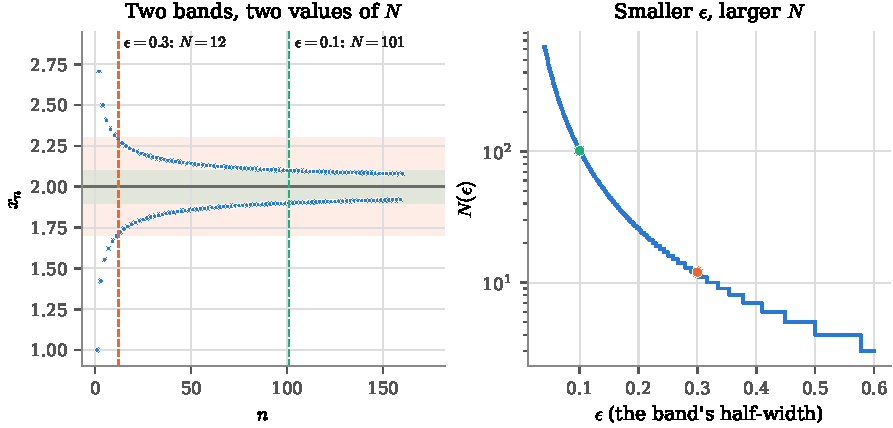
\includegraphics[width=\textwidth]{fig_tk_epsilon_n}
\caption{The $\epsilon$-$N$ definition as a game. Left: the sequence $x_n = 2 + (-1)^n/\sqrt{n}$ with the bands $2 \pm 0.3$ and $2 \pm 0.1$. Right: the smallest index $N$ that works, as a function of the tolerance $\epsilon$.}
\label{fig:tk-epsilon}
\end{figure}

\textbf{Where the book uses it.} \Cref{sec:conv-why} starts from this definition and explains why it cannot be applied directly to random variables; \cref{def:convp} keeps its shape but applies it to the \textit{probabilities} $\Pr(\abs{X_n - X} \geq \epsilon)$, which are ordinary numbers.
Every `$\to 0$' in a proof of convergence in probability is this definition applied to a sequence of numbers.

\textbf{Limits inside an expectation.} One further fact is used in the uniform law of large numbers of \cref{sec:proof-ulln} and, for an integral in place of an expectation, in \cref{ch:exp-families}: if random variables $W_r$ converge to $0$ as $r \to 0$ for every outcome, and all of them are bounded by one fixed random variable $G$ with $\E[G] < \infty$, then $\E[W_r] \to 0$ as well. This is the dominated convergence theorem. The bound is what makes it true: without it, a $W_r$ that is huge on a set of tiny probability can have an expectation that refuses to go to $0$ even though $W_r$ itself goes to $0$ at every outcome.

\section{Supremum and infimum}
\label{sec:math-sup}

The \textbf{maximum} of a set of numbers is its largest member.
Some sets have none: $\{1 - \frac{1}{n} : n = 1, 2, \ldots\}$ climbs toward $1$ and never reaches it.
The \textbf{supremum}, written $\sup$, is the least upper bound: the smallest number that no member exceeds.
For that set the supremum is $1$, which is not a member.
When a maximum exists it equals the supremum; the supremum exists more often, which is why proofs prefer it.
The \textbf{infimum}, $\inf$, is the greatest lower bound, and the same remarks apply with `minimum'.
\Cref{fig:tk-sup} shows both cases.
On the left, the set $\{1 - 1/n\}$ has no largest element, but $1$ is its least upper bound.
On the right, $x e^{-x}$ on $[0, 4]$ attains its supremum at $x = 1$ and its infimum at $x = 0$, so there $\sup = \max$ and $\inf = \min$; a continuous function on a closed, bounded interval always attains both. The same holds on any closed, bounded set in $\real^d$, such as a closed ball (the extreme value theorem).

\begin{figure}[htbp]
\centering
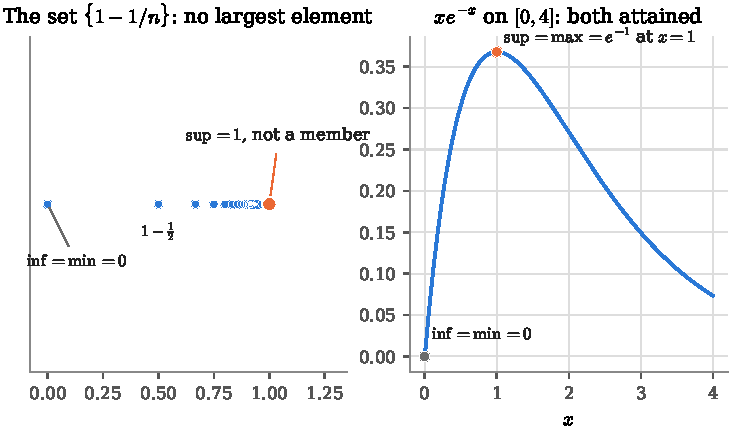
\includegraphics[width=\textwidth]{fig_tk_sup}
\caption{Left: the set $\{1 - 1/n : n = 1, 2, \ldots\}$ and its supremum $1$. Right: the function $x e^{-x}$ on $[0, 4]$.}
\label{fig:tk-sup}
\end{figure}

\textbf{Where the book uses it.} The conservative confidence interval of \cref{sec:ci-three-solutions} replaces $\sqrt{p(1-p)}$ by its supremum over $p \in (0,1)$, which is $\frac12$ and is attained; the subway version has $\sup_\lambda \lambda = \infty$, which is why no conservative interval exists there. \Cref{ch:estimators} mentions that a statistic may be defined through a $\sup$ or $\inf$; the maximum of a sample, $\max_i X_i$, is a maximum of finitely many numbers and causes no trouble. The proofs of consistency in \cref{thm:mle-consistent,thm:gof-family} use the extreme value theorem on a closed, bounded set of parameters.

\section{Sets, maps and one-to-one}
\label{sec:math-maps}

A \textbf{map} (or function) $f$ from a set $A$ to a set $B$ assigns to each element of $A$ exactly one element of $B$.
Its \textbf{image} is the set of elements of $B$ that are actually hit.
The map is \textbf{injective} (one-to-one) if different inputs always give different outputs: $a_1 \neq a_2$ implies $f(a_1) \neq f(a_2)$, or, turned around, $f(a_1) = f(a_2)$ implies $a_1 = a_2$.
An injective map can be undone: from the output you can recover the input.
For a function of one real variable the test is visual, the horizontal-line test of \cref{fig:tk-injective}: if some horizontal line crosses the graph twice, two inputs share an output and the map is not injective.
On the left of the figure, $\lambda \mapsto e^{-5\lambda}$ is strictly decreasing, so every height is hit once and $\lambda$ can be read off the output; this is the map of the censored-exponential example of \cref{ex:censored-expo}.
On the right, $x \mapsto x^2$ on $[-2, 2]$ hits the height $1$ twice, so the input cannot be recovered from the output.
A strictly increasing or strictly decreasing function always passes the test.

\begin{figure}[htbp]
\centering
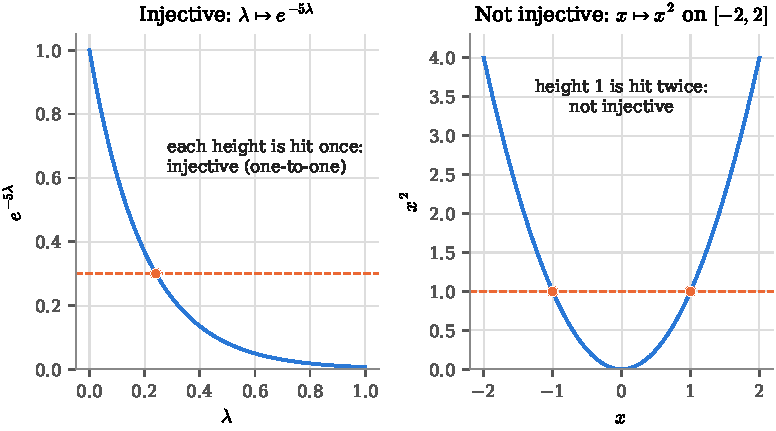
\includegraphics[width=\textwidth]{fig_tk_injective}
\caption{The horizontal-line test. Left: $\lambda \mapsto e^{-5\lambda}$, the map of the censored-exponential example of \cref{ex:censored-expo}. Right: $x \mapsto x^2$ on $[-2, 2]$.}
\label{fig:tk-injective}
\end{figure}

A \textbf{partition} of a set is a way of cutting it into pieces that do not overlap and together cover everything; any map partitions its domain into the sets of inputs that share an output.

\textbf{Where the book uses it.} Identifiability (\cref{def:identifiable}) is exactly the statement that the map $\theta \mapsto \Pr_\theta$ is injective; every identifiability argument in \cref{ch:models} is a horizontal-line test on that map. A statistic partitions the sample space (\cref{sec:est-reduction}).

\section{Indicator functions}
\label{sec:math-indicator}

The \textbf{indicator} of an event or a condition is the function that is $1$ when the condition holds and $0$ when it does not: $\ind(x \geq 5)$ is $0$ for $x < 5$ and $1$ from $5$ on.
It is the simplest random variable there is, a coin that comes up $1$ with probability $\Pr(\text{condition})$, and its expectation is that probability:
\[
\E[\ind(X \geq 5)] = 1 \cdot \Pr(X \geq 5) + 0 \cdot \Pr(X < 5) = \Pr(X \geq 5).
\]
That one line, \textit{the expectation of an indicator is a probability}, is how probabilities enter computations that are written with expectations, and how a sum of indicators becomes a count (the number of couples turning right is $\sum_i \ind(R_i = 1)$).
\Cref{fig:tk-indicator} draws the two sides of the line: on the left the indicator $\ind(x \geq 5)$, a step from $0$ to $1$; on the right, for $X \sim \Expo(0.16)$, its expectation as the shaded probability $\Pr(X \geq 5) = e^{-5 \times 0.16} = 0.45$.

\begin{figure}[htbp]
\centering
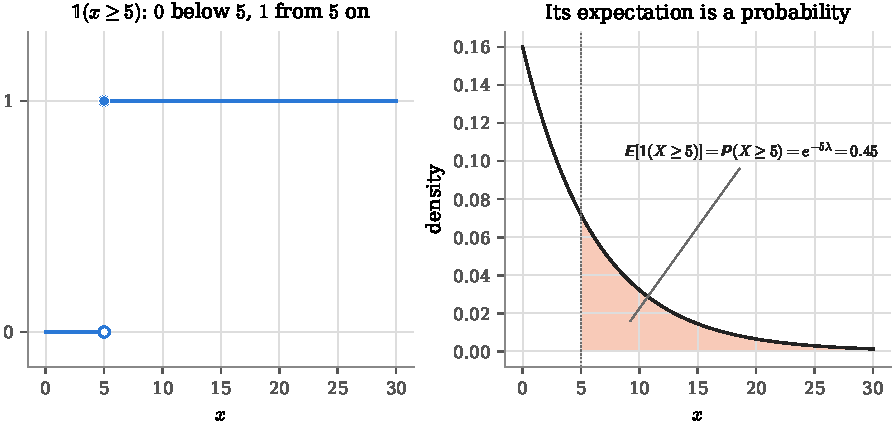
\includegraphics[width=\textwidth]{fig_tk_indicator}
\caption{Left: the indicator $\ind(x \geq 5)$ as a function of $x$. Right: the density of $X \sim \Expo(0.16)$, with the probability $\Pr(X \geq 5)$ shaded.}
\label{fig:tk-indicator}
\end{figure}

\textbf{Where the book uses it.} The CDF of a constant is a step function (\cref{ex:unif-shrinking}); the censored observations of \cref{ch:models} are indicators of the unobserved variable; the Strong Law in \cref{app:modes} counts failures with a sum of indicators; Markov's inequality below is proved with one.

\section{Random variables as functions, and `almost surely'}
\label{sec:math-rv}

A \textbf{random variable} is a function from the sample space (the set of possible outcomes of an experiment) to the real line.
\Cref{fig:tk-rv} draws the simplest case: the $36$ outcomes of two dice, and the function $X = $ `the sum'.
The probability $\Pr(X = 7)$ is the probability of the set of outcomes that $X$ sends to $7$: six of the $36$, so $\Pr(X = 7) = 6/36$ on the right of the figure.
Two random variables on the same sample space, say the sum $X$ and the larger die $Y$, are two functions of the \textit{same} outcome, which is what gives meaning to $X - Y$ and to `$X$ and $Y$ are close': you compare them outcome by outcome.
This is the viewpoint \cref{sec:conv-why} needs for a sequence of random variables, which is a sequence of functions on one sample space.

\begin{figure}[htbp]
\centering
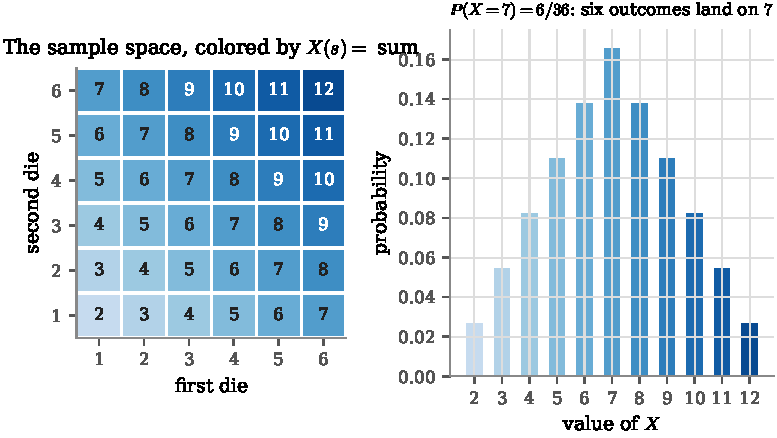
\includegraphics[width=\textwidth]{fig_tk_rv_function}
\caption{A random variable as a function on the sample space. Left: the $36$ outcomes of two dice, each colored by the value the function $X = $ `sum' assigns it. Right: the distribution of $X$ on the real line.}
\label{fig:tk-rv}
\end{figure}

Three phrases from probability theory appear in the book and mean less than they sound.
\begin{itemize}[nosep]
\item \textbf{Almost surely} means `with probability one'. A continuous random variable equals any particular number with probability zero, so `$X \neq 5$ almost surely' is true even though the outcome $X = 5$ is not impossible; the set of outcomes where a statement fails is allowed to be nonempty as long as it has probability zero. The book uses it in Hoeffding's inequality (`bounded almost surely': the probability of landing outside $[a, b]$ is zero) and in \cref{app:modes}.
\item \textbf{Measurable} (a measurable function, a measurable sample space) is the technical condition that makes probabilities of the relevant events well defined. Every function you can write down with formulas, limits, sums and integrals is measurable; the usual rule of thumb, that anything you can compute from the data is a statistic, is correct in practice. The book never needs more.
\item A \textbf{probability measure} (or distribution) assigns a probability to every event. A PMF or PDF is a recipe for one: sum or integrate it over the event. The two determine each other, and the book writes down families of distributions through their PMFs and PDFs (\cref{def:statmodel}).
\end{itemize}

\section{Densities, CDFs and quantiles}
\label{sec:math-density}

For a continuous random variable, \textbf{probability is area}: $\Pr(a \leq X \leq b)$ is the area under the density $f$ between $a$ and $b$.
The \textbf{CDF} $F(x) = \Pr(X \leq x)$ is the area accumulated up to $x$, so $\Pr(a \leq X \leq b) = F(b) - F(a)$, and $F$ is the antiderivative of $f$: $f = F'$.
The \textbf{quantile} reads the CDF backwards: given a probability $u$, the quantile is the $x$ with $F(x) = u$; the book's $q_\alpha$ is the case $u = 1 - \alpha$, indexed by the probability \textit{above} the cutoff.
\Cref{fig:tk-density} draws the three on one example, the standard Gaussian.
At the top, the shaded area under the density between $a = -1$ and $b = 1$ is $\Pr(a \leq X \leq b) = 0.683$.
At the bottom, the same probability is the rise of the CDF from $F(a)$ to $F(b)$, and reading the CDF sideways at $0.95$ gives the quantile $q_{0.05} = 1.645$ of \cref{sec:gauss-quantiles}.
The same three ideas work for a discrete random variable with sums in place of integrals: the PMF is the list of probabilities, the CDF the running total, and the CDF jumps at each possible value instead of rising smoothly.

\begin{figure}[htbp]
\centering
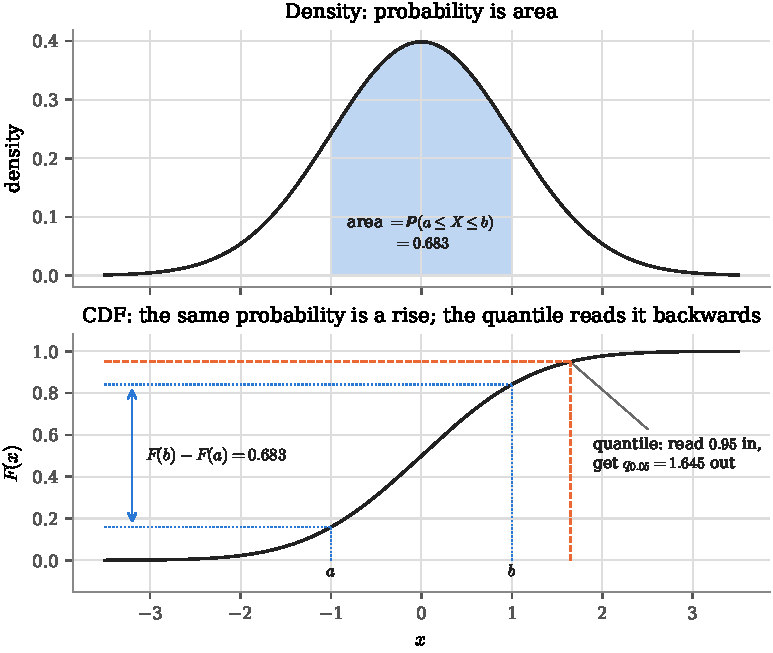
\includegraphics[width=0.78\textwidth]{fig_tk_density_cdf}
\caption{Density, CDF and quantile for $\Gauss(0,1)$. Top: the density, with the area between $a = -1$ and $b = 1$ shaded. Bottom: the CDF, with the rise from $F(a)$ to $F(b)$ and the quantile $q_{0.05}$ marked.}
\label{fig:tk-density}
\end{figure}

\textbf{Where the book uses it.} Convergence in distribution (\cref{def:convd}) compares CDFs, and the jumps of a discrete CDF are why only continuity points count. Every probability in \cref{ch:gaussian} is a CDF lookup. The density of a transformed variable, such as $aX + b$ or $X^2$, is found by writing its CDF and differentiating (\cref{sec:gauss-properties}, \cref{ch:models}).

\section{Three inequalities}
\label{sec:math-inequalities}

\textbf{The triangle inequality:} $\abs{x + y} \leq \abs{x} + \abs{y}$, and so $\abs{x - z} \leq \abs{x - y} + \abs{y - z}$: a detour through $y$ is never shorter than the direct distance.
Proofs use it to split an error into two pieces, for instance $\abs{T_n - \mu} \leq \abs{T_n - \E[T_n]} + \abs{\E[T_n] - \mu}$ in \cref{prop:shrinking-variance}: if the total is at least $\epsilon$, one of the two pieces is at least $\epsilon/2$.

\textbf{Markov's inequality:} if $Y \geq 0$ then $\Pr(Y \geq a) \leq \E[Y]/a$ for every $a > 0$.
The picture (\cref{fig:tk-inequalities}, left) is the proof: the step function $a \cdot \ind(Y \geq a)$ never exceeds $Y$, so its expectation, $a \Pr(Y \geq a)$, is at most $\E[Y]$.
A non-negative variable with a small mean is rarely large.

\textbf{Chebyshev's inequality:} for any random variable with finite variance, $\Pr(\abs{T - \E[T]} \geq \epsilon) \leq \var(T)/\epsilon^2$.
It is Markov's inequality applied to $Y = (T - \E[T])^2$ with $a = \epsilon^2$.
In standard-deviation units it says $\Pr(\abs{T - \E[T]} \geq k \sigma) \leq 1/k^2$ for every distribution whatsoever, which is both its strength (universal) and its weakness (loose: for a Gaussian the true two-standard-deviation tail is $0.046$, the bound says $0.25$).
The right of \cref{fig:tk-inequalities} draws the bound $1/k^2$ against the exact tail probabilities of a Gaussian and of an $\Expo(1)$ variable: the bound holds for every distribution and is far from tight for these two.

\begin{figure}[htbp]
\centering
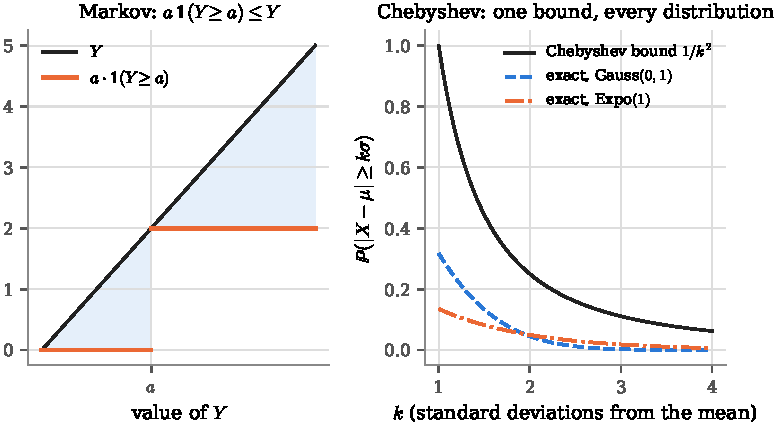
\includegraphics[width=\textwidth]{fig_tk_inequalities}
\caption{Left: $Y$ and the step function $a \cdot \ind(Y \geq a)$. Right: Chebyshev's bound $1/k^2$ against the exact probabilities $\Pr(\abs{T - \E[T]} \geq k\sigma)$ for a Gaussian $T$ and for $T \sim \Expo(1)$.}
\label{fig:tk-inequalities}
\end{figure}

\textbf{Where the book uses it.} The Law of Large Numbers (\cref{thm:wlln}) is Chebyshev's inequality with $n \to \infty$; the shrinking-variance criterion is the same with the triangle inequality in front; convergence in mean implies convergence in probability by Markov (\cref{app:modes}); Hoeffding's inequality (\cref{thm:hoeffding}) is the sharper cousin for bounded variables.

\section{Convex functions}
\label{sec:math-convex}

A function is \textbf{convex} if the chord joining any two points of its graph lies on or above the graph, and \textbf{concave} if every chord lies on or below (\cref{fig:tk-convex}).
For a function with a second derivative, convex means $g'' \geq 0$ (the slope keeps increasing) and concave means $g'' \leq 0$.
$x^2$, $e^x$ and $1/x$ on $(0, \infty)$ are convex; $\log x$ and $\sqrt{x}$ are concave; $\sin x$ is neither.
Averaging interacts with convexity in one direction only: for convex $g$, the average of $g$ over two points is at least $g$ of their average, which is the chord sitting above the curve at its midpoint.

\begin{figure}[htbp]
\centering
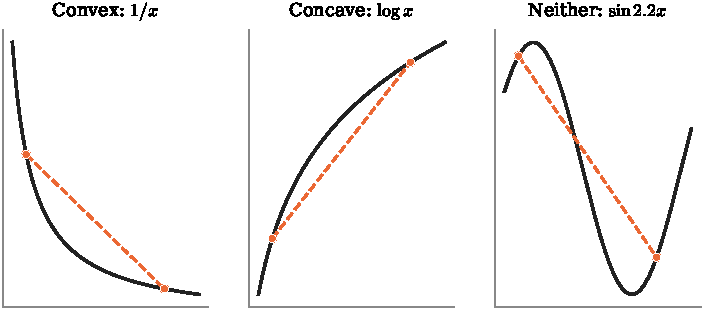
\includegraphics[width=\textwidth]{fig_tk_convex}
\caption{Convex: chords above the graph. Concave: chords below. Neither: a chord can cross the graph.}
\label{fig:tk-convex}
\end{figure}

\textbf{Where the book uses it.} Jensen's inequality (\cref{thm:jensen}) is the chord statement with the two-point average replaced by an expectation; it explains why $1/\bar{T}_n$ overestimates $\lambda$ and why $\sqrt{\cdot}$ of an unbiased estimator is biased (\cref{ch:estimators}). The quadratic in the solve interval of \cref{ch:confidence-intervals} is convex, which is why the inequality holds between its roots. Likelihoods in Part IV are maximized by finding where a concave function's slope is zero.

\section{Tangent lines, the mean value theorem and Taylor's expansion}
\label{sec:math-mvt}

The derivative $g'(\theta)$ is the slope of the tangent line to the graph of $g$ at $\theta$, and the tangent line $g(\theta) + g'(\theta)(x - \theta)$ is the best straight-line stand-in for $g$ near $\theta$.
Two facts make this precise.

\textbf{The mean value theorem.}
For a smooth $g$ and any $a < b$ there is a point $c$ between them where the tangent is parallel to the chord:
\[
g(b) - g(a) = g'(c) \, (b - a) \quad \text{for some } c \in (a, b).
\]
The change in $g$ over an interval equals the slope somewhere inside the interval times the interval's length: on the left of \cref{fig:tk-mvt}, the tangent at $c$ is parallel to the chord from $a$ to $b$.
You never learn where $c$ is, and you never need to: in the delta method it is squeezed between two points that converge to $\theta$, so $g'(c)$ converges to $g'(\theta)$.

\textbf{The first-order Taylor expansion.}
Near $\theta$,
\[
g(x) = g(\theta) + g'(\theta)(x - \theta) + \text{(an error of order } (x - \theta)^2),
\]
so on a window of width $h$ around $\theta$ the tangent line is wrong by about $h^2$, which is negligible compared with the $h$-sized changes along the line.
The right of \cref{fig:tk-mvt} draws this for $g(x) = 1/x$: the shaded error is tiny on the window $\theta \pm \sigma/\sqrt{n}$ where an estimator lives, which is why the delta method can treat $g$ as linear there.
Adding the next term, $\frac12 g''(\theta)(x - \theta)^2$, gives the second-order expansion, and it too has an exact form with an unknown in-between point, \textbf{Taylor's theorem with the Lagrange remainder}: for a twice differentiable $g$,
\[
g(b) = g(a) + g'(a)(b - a) + \tfrac12 g''(c)(b - a)^2 \quad \text{for some } c \text{ between } a \text{ and } b.
\]
At a maximum, where $g'(a) = 0$, it says that the drop from the top to $b$ is exactly half a squared distance times a curvature taken somewhere in between, which is the step behind the likelihood ratio test.
The pattern continues: for a $g$ with $k + 1$ derivatives, $g(x) = \sum_{i=0}^{k} \frac{1}{i!}g^{(i)}(\theta)(x - \theta)^i + (\text{an error of order } (x - \theta)^{k+1})$, where $g^{(i)}$ is the $i$th derivative and $g^{(0)} = g$.

\begin{figure}[htbp]
\centering
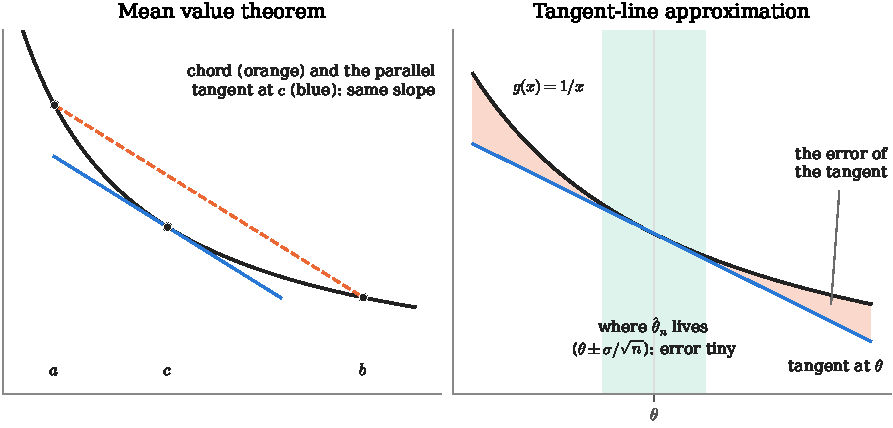
\includegraphics[width=\textwidth]{fig_tk_mvt_taylor}
\caption{Left: the mean value theorem, with the chord from $a$ to $b$ (orange) and the parallel tangent at $c$ (blue). Right: $g(x) = 1/x$ and its tangent line at $\theta$, with the error between them shaded over the window $\theta \pm \sigma/\sqrt{n}$.}
\label{fig:tk-mvt}
\end{figure}

\textbf{Where the book uses it.} The delta method (\cref{thm:delta}) is the mean value theorem followed by Slutsky's theorem; its intuition box is the tangent-line picture. The second-order expansion is behind the remark on $g'(\theta) = 0$ in \cref{sec:delta-method}, and Taylor's theorem with the Lagrange remainder proves Wilks' theorem in \cref{ch:wald-lrt}. \Cref{ex:gof-taylor} uses the terms of order three and four to compare $G^2$ with Pearson's statistic.

\section{Exponentials and logarithms}
\label{sec:math-explog}

Two facts about $e$ recur.
First, $(1 - x/n)^n \to e^{-x}$ as $n \to \infty$; the left of \cref{fig:tk-explog} shows the curves for $n = 1, 2, 5, 20$ climbing toward $e^{-x}$, each drawn up to $x = n$, where it reaches $0$. More generally $(1 + a/n)^n \to e^{a}$.
It is the step that turns the finite-$n$ formula in the maximum-of-uniforms proof (\cref{ex:max-unif}) into an exponential limit, and it reappears whenever a product of $n$ nearly-equal factors is pushed to the limit.
Second, the logarithm turns multiplication into addition, $\log(ab) = \log a + \log b$: on the right of \cref{fig:tk-explog}, equal ratios along the axis become equal steps up the curve, so a product becomes a sum.
A likelihood is a product of $n$ densities, a number so small it underflows a computer for moderate $n$; its logarithm is a sum of $n$ ordinary terms, and a sum of $n$ terms is what the Law of Large Numbers and the Central Limit Theorem know how to handle.
That is the entire reason Part IV works with log-likelihoods.
Because $\log$ is strictly increasing, maximizing the likelihood and maximizing the log-likelihood give the same answer.

\begin{figure}[htbp]
\centering
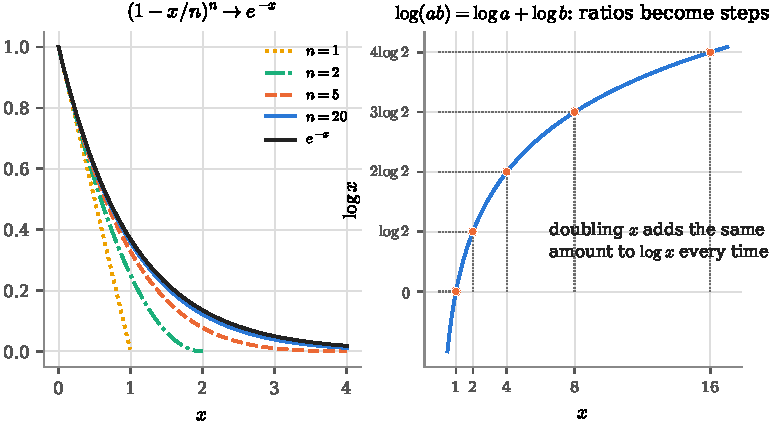
\includegraphics[width=\textwidth]{fig_tk_exp_log}
\caption{Left: $(1 - x/n)^n$ for $n = 1, 2, 5, 20$, each drawn up to $x = n$, and the limit $e^{-x}$. Right: the graph of the logarithm.}
\label{fig:tk-explog}
\end{figure}

\section{Orders of magnitude: how fast is `fast'}
\label{sec:math-rates}

The book keeps saying that an error is `of order $1/\sqrt{n}$', that a bound `goes to zero like $1/n$', or `exponentially fast'.
These are statements about how a quantity scales with $n$, ignoring constants.
\Cref{fig:tk-rates} draws the three rates that matter here on ordinary axes and on log-log axes, where a power law $n^{-c}$ is a straight line of slope $-c$ and an exponential bends away below every power law.
On ordinary axes the three look alike at first; on log-log axes $1/\sqrt{n}$ and $1/n$ are straight lines whose slopes are the exponents, and the exponential drops away below both.
Practical translation of each rate:
\begin{itemize}[nosep]
\item $1/\sqrt{n}$: four times the data halves the error; a hundred times the data buys one decimal place. This is the rate of every estimator built from an average and of every confidence interval in this book.
\item $1/n$: twice the data halves the error. Chebyshev's bound and the maximum-of-uniforms example have this rate; so does the bias of $1/\bar{T}_n$ in \cref{ch:estimators}, which is why the bias is swamped by the $1/\sqrt{n}$ standard error.
\item $e^{-cn}$: each fixed addition to $n$ multiplies the error by the same factor below $1$. Hoeffding's bound has this rate, which is why it overtakes Chebyshev's for large $n$ (\cref{fig:bounds}).
\end{itemize}

\begin{figure}[htbp]
\centering
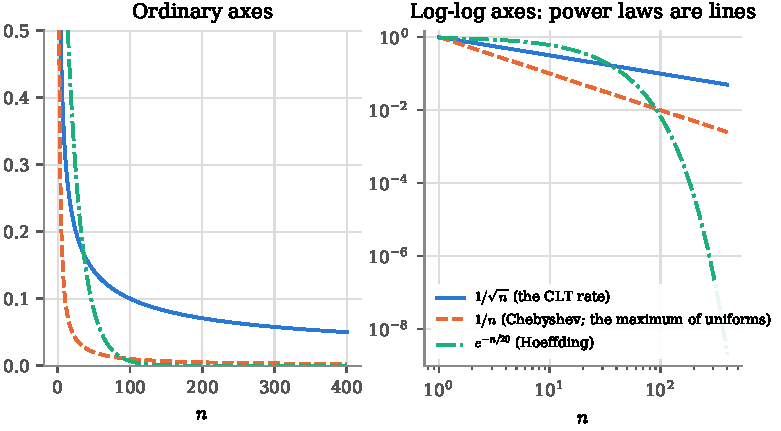
\includegraphics[width=\textwidth]{fig_tk_rates}
\caption{Three rates of decay, $1/\sqrt{n}$, $1/n$ and an exponential. Left: on ordinary axes. Right: on log-log axes.}
\label{fig:tk-rates}
\end{figure}

\section{Functions of several variables: gradient and Hessian}
\label{sec:math-multivar}

A parameter with several coordinates, like $(\mu, \sigma^2)$ for a Gaussian, turns a log-likelihood into a function of several variables, and maximizing it needs the several-variable versions of the derivative and the second derivative.

\textbf{Partial derivatives and the gradient.}
For $h(a, b)$, the partial derivative $\partial h/\partial a$ is the ordinary derivative in $a$ with $b$ held fixed: the slope of the surface walking in the $a$ direction.
The \textbf{gradient} collects them in a vector, $\nabla h = (\partial h/\partial a, \partial h/\partial b)$.
It points in the direction in which $h$ climbs fastest, it is perpendicular to the contour line through its point, and its length is the steepness of the climb.
On the left of \cref{fig:tk-gradient}, for the concave function $-(a^2 + ab + b^2)$, each arrow points uphill, perpendicular to the contour through its base, and the arrows shrink to nothing at the top, the one point where the gradient is $0$.
At the top of a hill the surface is flat in every direction, so the gradient is the zero vector: $\nabla h = 0$ is the first-order condition, one equation per coordinate.

\textbf{The Hessian and the second-derivative test.}
The \textbf{Hessian} is the matrix of second partial derivatives,
\[
\nabla^2 h = \begin{pmatrix} \partial^2 h/\partial a^2 & \partial^2 h/\partial a\,\partial b \\ \partial^2 h/\partial b\,\partial a & \partial^2 h/\partial b^2 \end{pmatrix},
\]
which is symmetric for the smooth functions of this book.
A zero gradient alone does not certify a maximum: the saddle $h(a, b) = a^2 - b^2$ has $\nabla h = 0$ at the origin, which is a minimum along $a$ and a maximum along $b$ (\cref{fig:tk-gradient}, right).
The second-derivative test settles it.
A symmetric matrix $H$ is \textbf{negative definite} if $u^\top H u < 0$ for every nonzero vector $u$: the function curves down in every direction.
If at a point where $\nabla h = 0$ the Hessian is negative definite, the point is a local maximum.
For a $2 \times 2$ Hessian, negative definite means the top-left entry is negative and the determinant is positive.
For the saddle the Hessian is $\begin{pmatrix} 2 & 0 \\ 0 & -2 \end{pmatrix}$, whose determinant is $-4$: not negative definite.
For $h(a, b) = -(a^2 + ab + b^2)$ it is $\begin{pmatrix} -2 & -1 \\ -1 & -2 \end{pmatrix}$, top-left $-2 < 0$, determinant $3 > 0$: negative definite, and the origin is the maximum.

\textbf{Concave in several variables.}
Along the line $\theta + tu$, the function $t \mapsto h(\theta + tu)$ has first derivative $\nabla h(\theta + tu)^\top u$ and second derivative $u^\top \nabla^2 h(\theta + tu)\, u$, by the chain rule.
Suppose the Hessian is negative definite at every point of a domain that contains the segment between any two of its points. Then the second derivative along every line is negative, so every slice through the function, in every direction, is strictly concave in one variable. If $\nabla h(\hat{\theta}) = 0$, the slice from $\hat{\theta}$ toward any other point $\theta$ has zero slope at $\hat{\theta}$, so by the one-variable result (\cref{prop:concave-max}) it is highest there: $h(\theta) < h(\hat{\theta})$. A point with zero gradient, if there is one, is the unique maximizer, exactly as in one variable.

\begin{figure}[htbp]
\centering
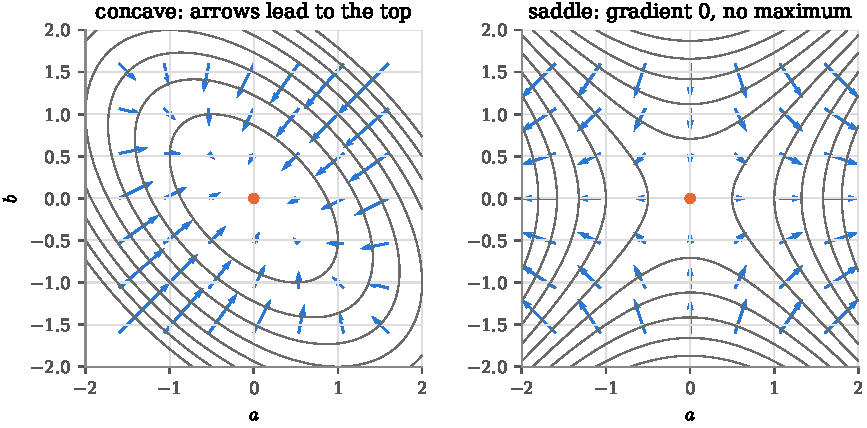
\includegraphics[width=\textwidth]{fig_tk_gradient}
\caption{Left: contours of $h(a, b) = -(a^2 + ab + b^2)$, with the gradient drawn as an arrow at a grid of points. Right: the saddle $h(a, b) = a^2 - b^2$.}
\label{fig:tk-gradient}
\end{figure}

\textbf{Where the book uses it.} The Gaussian maximum likelihood estimator (\cref{sec:lik-families}) is found by a two-step argument, and its Hessian at the maximum is negative definite; the EM algorithm (\cref{sec:lik-em}) maximizes in five coordinates; \cref{ch:mle-properties} turns the Hessian of the log-likelihood into the Fisher information matrix.

\section{Vectors of independent Gaussians and rotations}
\label{sec:math-gaussvec}

Cochran's theorem (\cref{thm:cochran}) rests on one fact: a vector of independent standard Gaussians looks the same after any rotation of the axes.
Three pieces of calculus and linear algebra make it precise.

\textbf{Joint densities.}
If $Z_1, \ldots, Z_n$ are independent continuous random variables with densities $f_1, \ldots, f_n$, the vector $Z = (Z_1, \ldots, Z_n)$ has the joint density $f(z) = f_1(z_1)\cdots f_n(z_n)$ on $\real^n$: the probability that $Z$ lands in a region is the integral of $f$ over it, and the product form is what independence means for densities.
Conversely, if a joint density factors as a product of a function of $z_1$ alone, a function of $z_2$ alone and so on, the coordinates are independent, each with the density its factor gives after normalizing.
For i.i.d.\ standard Gaussians,
\[
f(z) = \prod_{i=1}^n \frac{1}{\sqrt{2\pi}}e^{-z_i^2/2} = (2\pi)^{-n/2}\exp\Big(-\frac{\norm{z}^2}{2}\Big), \qquad \norm{z}^2 = z_1^2 + \cdots + z_n^2.
\]
The density depends on $z$ only through its length $\norm{z}$, so it is the same at every point of a sphere around the origin: the cloud of draws is round (\cref{fig:gaussrotation}).

\textbf{Orthogonal matrices.}
An $n \times n$ matrix $Q$ is \textbf{orthogonal} if $Q^\top Q = I$, which says that its columns are unit vectors perpendicular to each other: an orthonormal basis of $\real^n$ written as a matrix. Since $Q$ is square, $Q^\top Q = I$ makes $Q^\top$ the inverse of $Q$, so $QQ^\top = I$ as well: the rows are orthonormal too, and $Q^\top$ is itself orthogonal.
Multiplying by $Q$ rotates (and possibly reflects) the axes.
Two consequences: $Q$ preserves lengths, $\norm{Qz}^2 = (Qz)^\top(Qz) = z^\top Q^\top Q z = \norm{z}^2$, and $\det Q = \pm 1$, since $\det(Q^\top Q) = (\det Q)^2 = 1$.
Any unit vector $u_1$ can be made the first row of an orthogonal matrix: extend it to a basis of $\real^n$ and run the Gram--Schmidt process, which subtracts from each new vector its components along the previous ones and normalizes, producing an orthonormal basis $u_1, \ldots, u_n$ that keeps $u_1$ as it is; the same process keeps any orthonormal $u_1, \ldots, u_k$ as the first $k$ rows.
The proof of \cref{thm:cochran} uses $u_1 = (1, \ldots, 1)/\sqrt{n}$.

\textbf{Change of variables for a linear map.}
If $Z$ has density $f$ on $\real^n$ and $A$ is an invertible $n \times n$ matrix, then $Y = AZ$ has density
\[
f_Y(y) = \frac{f(A^{-1}y)}{\abs{\det A}}.
\]
This is the substitution rule of multivariable calculus: a linear map multiplies every volume by $\abs{\det A}$, so the probability $f(z)\,\mathrm{d}z$ of a small box around $z$ is spread over a box of volume $\abs{\det A}\,\mathrm{d}z$ around $y = Az$.
For $n = 1$ it is the familiar $f_Y(y) = f(y/a)/\abs{a}$ for $Y = aZ$, the affine property of \cref{ch:gaussian}.

\textbf{Rotation invariance.}
Put the three together.
Let $Z$ have i.i.d.\ $\Gauss(0,1)$ coordinates and $Q$ be orthogonal, and set $Y = QZ$.
Then $A^{-1} = Q^{-1} = Q^\top$, $\abs{\det Q} = 1$, and $\norm{Q^\top y} = \norm{y}$, so
\[
f_Y(y) = (2\pi)^{-n/2}\exp\Big(-\frac{\norm{Q^\top y}^2}{2}\Big) = (2\pi)^{-n/2}\exp\Big(-\frac{\norm{y}^2}{2}\Big) = \prod_{i=1}^n \frac{1}{\sqrt{2\pi}}e^{-y_i^2/2}.
\]
The density of $Y$ is the same product, so $Y_1, \ldots, Y_n$ are again i.i.d.\ $\Gauss(0,1)$, and $\norm{Y} = \norm{Z}$.
In words: rotate a round Gaussian cloud and you get the same round Gaussian cloud, with the new coordinates as independent as the old ones.
\Cref{ex:t-cochran-two} does the computation by hand for $n = 2$ and the $45^\circ$ rotation.

\textbf{Where the book uses it.} \Cref{thm:cochran} rotates the standardized data so that one coordinate is $\sqrt{n}\bar{Z}_n$ and the others carry the deviations; \cref{thm:pearson} rotates the standardized deviations of the counts with an orthogonal matrix whose first row is $(\sqrt{p^0_1}, \ldots, \sqrt{p^0_K})$, the direction in which those deviations cannot move; \cref{thm:reg-exact} rotates the errors of a regression with the first two axes along $(1, \ldots, 1)$ and along the centered explanatory values; \cref{ch:regression-multi} uses the same rotation with the regressors' subspace in place of the line through $(1, \ldots, 1)$.

\section{Gaussian vectors with a covariance matrix}
\label{sec:math-gaussquad}

The limits in \cref{ch:mle-properties,ch:mom-mestimation,ch:wald-lrt} are Gaussian vectors whose coordinates have different variances and are correlated.
This entry says what such a vector is, building on the round Gaussian cloud of the previous entry, and proves the facts the book uses about it.

\textbf{Covariance matrices.}
For a random vector $Z = (Z_1, \ldots, Z_d)$ with finite variances, the covariance matrix $\cov(Z)$ has entries $\cov(Z_j, Z_k)$, with the variances on the diagonal.
For a matrix $B$, $\cov(BZ) = B\,\cov(Z)\,B^\top$: each entry is the covariance of two linear combinations of the $Z_j$, expanded term by term.
A covariance matrix $\Sigma$ is symmetric, and $a^\top\Sigma a = \var(a^\top Z) \geq 0$ for every vector $a$.
It is \textbf{positive definite} when $a^\top\Sigma a > 0$ for every $a \neq 0$, that is, when no nonzero linear combination of the coordinates is constant; a positive definite matrix is invertible, since $\Sigma a = 0$ would give $a^\top\Sigma a = 0$.
Conversely, an invertible covariance matrix is positive definite.
If $a^\top\Sigma a = \var(a^\top Z) = 0$, then $a^\top Z$ is constant, so $(\Sigma a)_j = \cov(Z_j, a^\top Z) = 0$ for every $j$; that is, $\Sigma a = 0$, and invertibility forces $a = 0$.
The inverse of a positive definite matrix is positive definite too: for $a \neq 0$, $b = \Sigma^{-1}a$ is not $0$, and $a^\top\Sigma^{-1}a = b^\top\Sigma b > 0$.
The Fisher information matrix is the covariance matrix of the score (\cref{def:fisher}), so when it is invertible it is positive definite, and so is its inverse.

\textbf{Definition.}
Let $m \in \real^d$ and let $\Sigma$ be a symmetric positive definite $d \times d$ matrix.
A random vector $Z$ has the \textbf{Gaussian distribution} $\Gauss_d(m, \Sigma)$ if it has the distribution of $m + AW$, where $W$ has $d$ independent $\Gauss(0, 1)$ coordinates and $A$ is an invertible $d \times d$ matrix with $AA^\top = \Sigma$.
The definition concerns only the distribution of $Z$, which is all that a limit in distribution, such as the one in the Central Limit Theorem, delivers.
Such an $A$ exists for every positive definite $\Sigma$; one choice is the lower-triangular matrix of the Cholesky factorization, a standard result of linear algebra, and for $d = 2$ it is explicit: for $\Sigma = \begin{pmatrix} a & b \\ b & c\end{pmatrix}$, $A = \begin{pmatrix} \sqrt{a} & 0 \\ b/\sqrt{a} & \sqrt{c - b^2/a}\end{pmatrix}$.
$\cov(Z) = A\,\cov(W)A^\top = AA^\top = \Sigma$, and every nonzero linear combination $a^\top Z$ has the distribution of $a^\top m + (A^\top a)^\top W$, a sum of independent Gaussians plus a constant, so it is $\Gauss(a^\top m, a^\top\Sigma a)$ by the sum rule and the affine property of \cref{ch:gaussian}.
That is the description of $\Gauss_d$ used in the recall lines of \cref{ch:mom-mestimation}.
(Conversely, a vector all of whose linear combinations are Gaussian, with positive definite covariance matrix, has this form; the proof uses characteristic functions, which this book does not develop, and nothing in the book needs it.)

\textbf{The distribution depends on $A$ only through $\Sigma$.}
By the change of variables formula of the previous entry, with $f$ the density of $W$,
\[
f_Z(z) = \frac{f\big(A^{-1}(z - m)\big)}{\abs{\det A}} = \frac{1}{(2\pi)^{d/2}\abs{\det A}}\exp\Big(-\tfrac12\norm{A^{-1}(z - m)}^2\Big).
\]
Now $\norm{A^{-1}(z - m)}^2 = (z - m)^\top(A^{-1})^\top A^{-1}(z - m) = (z - m)^\top(AA^\top)^{-1}(z - m)$, and $\abs{\det A} = \sqrt{\det(AA^\top)}$, so
\[
f_Z(z) = \frac{1}{(2\pi)^{d/2}\sqrt{\det\Sigma}}\exp\Big(-\tfrac12(z - m)^\top\Sigma^{-1}(z - m)\Big),
\]
a formula with only $m$ and $\Sigma$ in it: two choices of $A$ with the same $AA^\top$ give the same distribution.
For $d = 1$ it is the Gaussian density of \cref{ch:gaussian}.
The contours of the density are the ellipses $(z - m)^\top\Sigma^{-1}(z - m) = \text{constant}$, drawn in \cref{fig:gaussquad}.

\textbf{Linear maps.}
If $Z \sim \Gauss_d(m, \Sigma)$ and $B$ is a $k \times d$ matrix of rank $k$ (its rows are linearly independent), then $BZ \sim \Gauss_k(Bm, B\Sigma B^\top)$.
To see it, note that $BZ$ has the distribution of $Bm + CW$ with $C = BA$, a $k \times d$ matrix of rank $k$, since $A$ is invertible.
Run the Gram--Schmidt process on the rows of $C$ to get orthonormal vectors $q_1, \ldots, q_k$ spanning the same space, and let $Q_1$ be the $k \times d$ matrix with these rows.
Each row of $C$ is a combination of $q_1, \ldots, q_k$, so $C = LQ_1$ with $L = CQ_1^\top$, a $k \times k$ matrix; it is invertible, since $k = \mathrm{rank}\,C = \mathrm{rank}(LQ_1) \leq \mathrm{rank}\,L$.
Extend $q_1, \ldots, q_k$ to a basis of $\real^d$ and continue the Gram--Schmidt process, as in the previous entry, to get an orthogonal matrix $Q$ whose first $k$ rows are $q_1, \ldots, q_k$.
By rotation invariance $QW$ has independent standard Gaussian coordinates, and $W' = Q_1W$ is its first $k$ of them.
So $BZ$ has the distribution of $Bm + LW'$, with $L$ invertible and $LL^\top = LQ_1Q_1^\top L^\top = CC^\top = B\Sigma B^\top$, which is the definition.

\textbf{The quadratic form.}
If $Z \sim \Gauss_d(m, \Sigma)$, then $(Z - m)^\top\Sigma^{-1}(Z - m)$ has the distribution of $W^\top A^\top(AA^\top)^{-1}AW = W^\top W$, which is $\chi^2_d$ (\cref{lem:gauss-quadform}): the squared distance from the center in units of the noise, which \cref{fig:gaussquad} draws.

\textbf{Where the book uses it.} The multivariate CLT and the asymptotic normality of estimators with several coordinates (\cref{ch:limit-tools,ch:mle-properties,ch:mom-mestimation}) have $\Gauss_d$ limits when their covariance matrices are positive definite. The quadratic form gives the chi-squared limits of Wald's, the likelihood ratio and the score tests (\cref{ch:wald-lrt}), and the linear-map rule gives the common limit of all three with nuisance parameters (\cref{thm:three-nuisance}). The vector of counts in \cref{ch:gof}, whose coordinates add up to $n$, has a covariance matrix that is not positive definite; that chapter rotates the standardized deviations of the counts so that the direction in which they cannot move is one coordinate and sets it aside (\cref{thm:pearson}), and for the three tests drops one category (\cref{sec:gof-score}); either way the covariance matrix that remains is positive definite.

\section{Conditional distributions and conditional expectation}
\label{sec:math-condexp}

For a pair $(X, Y)$ with a joint density $h(x, y)$, the \textbf{marginal density} of $X$ is $h(x) = \int h(x, y)\,\mathrm{d}y$, and wherever $h(x) > 0$ the \textbf{conditional density} of $Y$ given $X = x$ is
\[
h(y \mid x) = \frac{h(x, y)}{h(x)}:
\]
the slice of the joint density along the vertical line at $x$, rescaled so that it integrates to $1$.
For discrete pairs, PMFs replace densities and sums replace integrals: $\Pr(Y = y \mid X = x) = \Pr(X = x, Y = y)/\Pr(X = x)$.
The \textbf{conditional expectation} $\E[Y \mid X = x] = \int y\,h(y \mid x)\,\mathrm{d}y$ is the mean of that slice, one number for each $x$.
\Cref{fig:tk-condexp} draws the simplest case: two dice, $X$ the first and $Y$ the sum. Given $X = x$, the sum is $x + d$ with $d = 1, \ldots, 6$ equally likely, so $\E[Y \mid X = x] = x + 3.5$.

\begin{figure}[htbp]
\centering
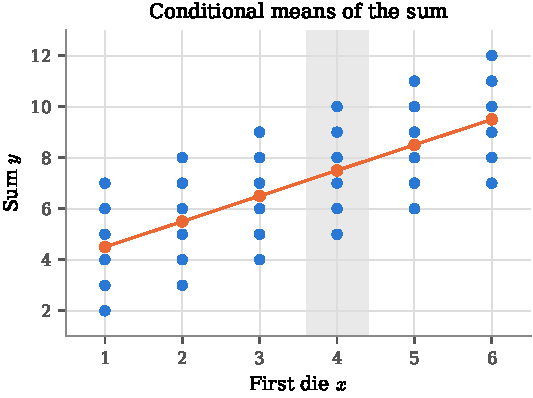
\includegraphics[width=0.6\textwidth]{fig_tk_condexp}
\caption{Two dice: the $36$ equally likely outcomes as points (first die, sum), and the conditional means of the sum given the first die (orange); the shaded column holds the six outcomes with first die $4$.}
\label{fig:tk-condexp}
\end{figure}

Writing $f(x) = \E[Y \mid X = x]$, the random variable $f(X)$, the conditional mean evaluated at the observed $X$, is written $\E[Y \mid X]$. Three facts handle it.
\begin{itemize}[nosep]
\item \textbf{The tower property}: $\E\big[\E[Y \mid X]\big] = \E[Y]$. For densities, $\E[f(X)] = \int f(x)h(x)\,\mathrm{d}x = \iint y\,h(y \mid x)h(x)\,\mathrm{d}y\,\mathrm{d}x = \iint y\,h(x, y)\,\mathrm{d}y\,\mathrm{d}x = \E[Y]$. For the dice, the average of $x + 3.5$ over $x = 1, \ldots, 6$ is $7$, the mean of the sum.
\item \textbf{Taking out what is known}: $\E[g(X)Y \mid X] = g(X)\E[Y \mid X]$ for any function $g$ with $\E\abs{g(X)Y} < \infty$: once $X = x$ is fixed, $g(x)$ is a constant and comes out of the mean of the slice. With the tower property, $\E[g(X)Y] = \E\big[g(X)\E[Y \mid X]\big]$.
\item \textbf{Conditional variance}: $\var(Y \mid X = x) = \E[Y^2 \mid X = x] - \big(\E[Y \mid X = x]\big)^2$ is the variance of the slice, so it is non-negative; hence $\E[Y \mid X]^2 \leq \E[Y^2 \mid X]$, and by the tower property $\E\big[\E[Y \mid X]^2\big] \leq \E[Y^2]$.
\end{itemize}

\textbf{Where the book uses it.} The posterior of \cref{ch:bayes-intro} is a conditional density of the parameter given the data; the regression function of \cref{ch:regression-uni} is a conditional expectation, and the proof that it is the best predictor (\cref{thm:best-predictor}) uses all three facts.

\section{Matrices, rank and projections}
\label{sec:math-matrices}

\Cref{ch:regression-multi} writes $n$ regression equations as one, $Y = X\beta + \epsilon$, and solves them by geometry.
This entry collects the linear algebra that takes.

\textbf{Vectors and matrices.}
A vector $v \in \real^n$ is a column of $n$ numbers; $v^\top$ is the same numbers as a row, so $u^\top v = \sum_i u_iv_i$ is a number, the inner product, and $\norm{v}^2 = v^\top v$ is the squared length.
Two vectors are \textbf{perpendicular} (orthogonal) when $u^\top v = 0$, and then $\norm{u + v}^2 = \norm{u}^2 + \norm{v}^2$ (Pythagoras: the cross term $2u^\top v$ vanishes).
An $n \times p$ matrix $X$ sends $\beta \in \real^p$ to $X\beta \in \real^n$, which is the combination $\beta_1x_{(1)} + \cdots + \beta_px_{(p)}$ of the columns of $X$ with the entries of $\beta$ as weights.
The transpose rule $(AB)^\top = B^\top A^\top$ and the inverse rule $(AB)^{-1} = B^{-1}A^{-1}$ hold whenever the products and inverses exist; the \textbf{trace} $\mathrm{tr}(A)$ of a square matrix is the sum of its diagonal entries, $\mathrm{tr}(AB) = \mathrm{tr}(BA)$ whenever both products are square, and $\mathrm{tr}$ is linear, so it passes through expectations.

\textbf{Column space and rank.}
The \textbf{column space} of $X$ is the set of all vectors $X\beta$, a subspace of $\real^n$ (closed under sums and multiples).
The columns are \textbf{linearly independent} when $X\beta = 0$ only for $\beta = 0$, that is, when no column is a combination of the others; then every vector in the column space is $X\beta$ for exactly one $\beta$, and the column space has dimension $p$.
The \textbf{rank} of $X$ is the dimension of its column space, so `rank $p$' with $p \leq n$ means the columns are independent.
Independent columns make $X^\top X$ invertible: $X^\top Xa = 0$ gives $a^\top X^\top Xa = \norm{Xa}^2 = 0$, so $Xa = 0$ and $a = 0$.

\textbf{Orthogonal projection.}
Let $S$ be a subspace of $\real^n$ of dimension $d$. The Gram--Schmidt process of \cref{sec:math-gaussvec}, fed a basis of $S$ and then vectors completing it to a basis of $\real^n$, gives an orthonormal basis $u_1, \ldots, u_n$ of $\real^n$ whose first $d$ vectors span $S$; fed a basis of a smaller subspace $S_0 \subset S$ first, it gives one adapted to the chain $S_0 \subset S \subset \real^n$.
Every $y$ then splits as $y = s + r$ with $s = \sum_{k \leq d}(u_k^\top y)u_k \in S$ and $r = \sum_{k > d}(u_k^\top y)u_k$ perpendicular to every vector of $S$, and uniquely, since two such splits would differ by a vector of $S$ perpendicular to $S$, which is $0$; $s$ is the \textbf{orthogonal projection} of $y$ onto $S$, and it is the point of $S$ closest to $y$, since for any $s' \in S$, $\norm{y - s'}^2 = \norm{r}^2 + \norm{s - s'}^2 \geq \norm{r}^2$ by Pythagoras.
\Cref{fig:tk-projection} draws the case of a line.
The map $y \mapsto s$ is linear, so it is a matrix $P$, with $P^2 = P$ (projecting twice changes nothing) and $P^\top = P$; for $S$ the column space of a rank-$p$ matrix $X$, the condition that $y - Py$ be perpendicular to every column reads $X^\top(y - Xb) = 0$, whose solution $b = (X^\top X)^{-1}X^\top y$ gives
\[
P = X(X^\top X)^{-1}X^\top, \qquad \mathrm{tr}(P) = \mathrm{tr}\big((X^\top X)^{-1}X^\top X\big) = p.
\]
$I - P$ is the projection onto the \textbf{orthogonal complement} of $S$, the vectors perpendicular to $S$, a subspace of dimension $n - p$.
In the adapted basis, $P = \sum_{k \leq d}u_ku_k^\top$, so if $S_0 \subset S$ are nested subspaces of dimensions $d_0 \leq d$ with projections $P_0 = \sum_{k \leq d_0}u_ku_k^\top$ and $P$, then $PP_0 = P_0$, and $P - P_0 = \sum_{d_0 < k \leq d}u_ku_k^\top$ is the projection onto the span of $u_{d_0+1}, \ldots, u_d$, the part of $S$ perpendicular to $S_0$, of dimension $d - d_0$.

\begin{figure}[htbp]
\centering
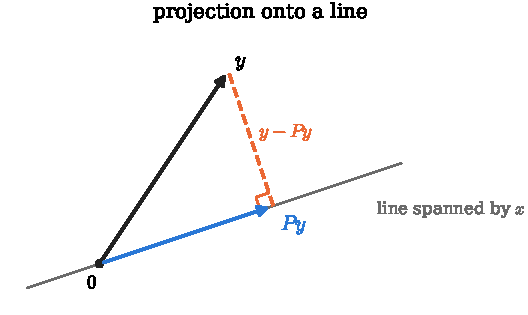
\includegraphics[width=0.5\textwidth]{fig_tk_projection}
\caption{Orthogonal projection onto a line: the vector $y$ (black), the line spanned by $x$ (gray), the projection $Py$ (blue) and the residual $y - Py$ (orange, dashed), perpendicular to the line.}
\label{fig:tk-projection}
\end{figure}

\textbf{Where the book uses it.} Least squares is the projection of the response onto the column space of the design matrix (\cref{thm:mreg-lse}); the residual sum of squares has $n - p$ degrees of freedom because $I - P$ projects onto an $(n - p)$-dimensional space (\cref{thm:mreg-exact}); the $F$-test splits the column space into nested pieces (\cref{thm:mreg-ftest}); and full rank is the identifiability of the regression model (\cref{ch:models}).

\section{To be added with later chapters}
\label{sec:math-later}

Eigenvalues and eigenvectors (for \cref{ch:pca}).
